
%(BEGIN_QUESTION)
% Copyright 2010, Tony R. Kuphaldt, released under the Creative Commons Attribution License (v 1.0)
% This means you may do almost anything with this work of mine, so long as you give me proper credit

PT-56 measures gas pressure inside a chemical reactor vessel over a range of 0 to 25 PSI, through a remote seal:

$$\includegraphics[width=15.5cm]{i03709x01.eps}$$

The pressure transmitter is presently mounted 14 feet below the remote seal, with a fill fluid density of 66.8 lb/ft$^{3}$.  A decision is made to relocate this transmitter to a more accessible spot, 4 feet above where it presently is, and you must decide how to reconfigure the transmitter to work properly in this new location.  Based on this information, answer the following questions:

\vskip 10pt

For new location: LRV = \underbar{\hskip 50pt} PSI \hskip 30pt  URV = \underbar{\hskip 50pt} PSI

\vskip 10pt

Will this re-location necessitate a {\it re-calibration} (sensor trim) of PT-56, or merely a {\it re-ranging}?

\vskip 10pt

Does the re-location necessitate a change in controller action from direct to reverse, or vice-versa?

\vskip 10pt

Assuming an air-to-open PV-56 control valve, does PIC-56 need to be {\it direct} or {\it reverse} acting?

\underbar{file i03709}
%(END_QUESTION)





%(BEGIN_ANSWER)

\noindent
(2 points each)

LRV = \underbar{\bf 4.64} PSI \hskip 30pt  URV = \underbar{\bf 29.64} PSI

\vskip 10pt

\noindent
(2 points)

This re-location will merely necessitate a {\bf re-ranging} and not a re-calibration of the transmitter.

\vskip 10pt

\noindent
(2 points)

The re-location does {\bf not} necessitate any change in controller action.

\vskip 10pt

\noindent
(2 points)

Assuming an air-to-open PV-56 control valve, PIC-56 needs to be {\bf reverse} acting.


%(END_ANSWER)





%(BEGIN_NOTES)

{\bf This question is intended for exams only and not worksheets!}.

%(END_NOTES)


